% Options for packages loaded elsewhere
\PassOptionsToPackage{unicode}{hyperref}
\PassOptionsToPackage{hyphens}{url}
\PassOptionsToPackage{dvipsnames,svgnames,x11names}{xcolor}
\documentclass[
  11pt,
  letterpaper,
]{article}
\usepackage{xcolor}
\usepackage[margin=1in]{geometry}
\usepackage{amsmath,amssymb}
\setcounter{secnumdepth}{-\maxdimen} % remove section numbering
\usepackage{iftex}
\ifPDFTeX
  \usepackage[T1]{fontenc}
  \usepackage[utf8]{inputenc}
  \usepackage{textcomp} % provide euro and other symbols
\else % if luatex or xetex
  \usepackage{unicode-math} % this also loads fontspec
  \defaultfontfeatures{Scale=MatchLowercase}
  \defaultfontfeatures[\rmfamily]{Ligatures=TeX,Scale=1}
\fi
\usepackage{lmodern}
\usepackage{newunicodechar}
\newunicodechar{≥}{\ensuremath{\geq}}
\newunicodechar{≤}{\ensuremath{\leq}}
\ifPDFTeX\else
  % xetex/luatex font selection
\fi
% Use upquote if available, for straight quotes in verbatim environments
\IfFileExists{upquote.sty}{\usepackage{upquote}}{}
\IfFileExists{microtype.sty}{% use microtype if available
  \usepackage[]{microtype}
  \UseMicrotypeSet[protrusion]{basicmath} % disable protrusion for tt fonts
}{}
\usepackage{setspace}
\makeatletter
\@ifundefined{KOMAClassName}{% if non-KOMA class
  \IfFileExists{parskip.sty}{%
    \usepackage{parskip}
  }{% else
    \setlength{\parindent}{0pt}
    \setlength{\parskip}{6pt plus 2pt minus 1pt}}
}{% if KOMA class
  \KOMAoptions{parskip=half}}
\makeatother
\usepackage{color}
\usepackage{fancyvrb}
\newcommand{\VerbBar}{|}
\newcommand{\VERB}{\Verb[commandchars=\\\{\}]}
\DefineVerbatimEnvironment{Highlighting}{Verbatim}{commandchars=\\\{\}}
% Add ',fontsize=\small' for more characters per line
\newenvironment{Shaded}{}{}
\newcommand{\AlertTok}[1]{\textcolor[rgb]{1.00,0.00,0.00}{\textbf{#1}}}
\newcommand{\AnnotationTok}[1]{\textcolor[rgb]{0.38,0.63,0.69}{\textbf{\textit{#1}}}}
\newcommand{\AttributeTok}[1]{\textcolor[rgb]{0.49,0.56,0.16}{#1}}
\newcommand{\BaseNTok}[1]{\textcolor[rgb]{0.25,0.63,0.44}{#1}}
\newcommand{\BuiltInTok}[1]{\textcolor[rgb]{0.00,0.50,0.00}{#1}}
\newcommand{\CharTok}[1]{\textcolor[rgb]{0.25,0.44,0.63}{#1}}
\newcommand{\CommentTok}[1]{\textcolor[rgb]{0.38,0.63,0.69}{\textit{#1}}}
\newcommand{\CommentVarTok}[1]{\textcolor[rgb]{0.38,0.63,0.69}{\textbf{\textit{#1}}}}
\newcommand{\ConstantTok}[1]{\textcolor[rgb]{0.53,0.00,0.00}{#1}}
\newcommand{\ControlFlowTok}[1]{\textcolor[rgb]{0.00,0.44,0.13}{\textbf{#1}}}
\newcommand{\DataTypeTok}[1]{\textcolor[rgb]{0.56,0.13,0.00}{#1}}
\newcommand{\DecValTok}[1]{\textcolor[rgb]{0.25,0.63,0.44}{#1}}
\newcommand{\DocumentationTok}[1]{\textcolor[rgb]{0.73,0.13,0.13}{\textit{#1}}}
\newcommand{\ErrorTok}[1]{\textcolor[rgb]{1.00,0.00,0.00}{\textbf{#1}}}
\newcommand{\ExtensionTok}[1]{#1}
\newcommand{\FloatTok}[1]{\textcolor[rgb]{0.25,0.63,0.44}{#1}}
\newcommand{\FunctionTok}[1]{\textcolor[rgb]{0.02,0.16,0.49}{#1}}
\newcommand{\ImportTok}[1]{\textcolor[rgb]{0.00,0.50,0.00}{\textbf{#1}}}
\newcommand{\InformationTok}[1]{\textcolor[rgb]{0.38,0.63,0.69}{\textbf{\textit{#1}}}}
\newcommand{\KeywordTok}[1]{\textcolor[rgb]{0.00,0.44,0.13}{\textbf{#1}}}
\newcommand{\NormalTok}[1]{#1}
\newcommand{\OperatorTok}[1]{\textcolor[rgb]{0.40,0.40,0.40}{#1}}
\newcommand{\OtherTok}[1]{\textcolor[rgb]{0.00,0.44,0.13}{#1}}
\newcommand{\PreprocessorTok}[1]{\textcolor[rgb]{0.74,0.48,0.00}{#1}}
\newcommand{\RegionMarkerTok}[1]{#1}
\newcommand{\SpecialCharTok}[1]{\textcolor[rgb]{0.25,0.44,0.63}{#1}}
\newcommand{\SpecialStringTok}[1]{\textcolor[rgb]{0.73,0.40,0.53}{#1}}
\newcommand{\StringTok}[1]{\textcolor[rgb]{0.25,0.44,0.63}{#1}}
\newcommand{\VariableTok}[1]{\textcolor[rgb]{0.10,0.09,0.49}{#1}}
\newcommand{\VerbatimStringTok}[1]{\textcolor[rgb]{0.25,0.44,0.63}{#1}}
\newcommand{\WarningTok}[1]{\textcolor[rgb]{0.38,0.63,0.69}{\textbf{\textit{#1}}}}
\usepackage{longtable,booktabs,array}
\newcounter{none} % for unnumbered tables
\usepackage{calc} % for calculating minipage widths
% Correct order of tables after \paragraph or \subparagraph
\usepackage{etoolbox}
\makeatletter
\patchcmd\longtable{\par}{\if@noskipsec\mbox{}\fi\par}{}{}
\makeatother
% Allow footnotes in longtable head/foot
\IfFileExists{footnotehyper.sty}{\usepackage{footnotehyper}}{\usepackage{footnote}}
\makesavenoteenv{longtable}
\usepackage{graphicx}
\makeatletter
\newsavebox\pandoc@box
\newcommand*\pandocbounded[1]{% scales image to fit in text height/width
  \sbox\pandoc@box{#1}%
  \Gscale@div\@tempa{\textheight}{\dimexpr\ht\pandoc@box+\dp\pandoc@box\relax}%
  \Gscale@div\@tempb{\linewidth}{\wd\pandoc@box}%
  \ifdim\@tempb\p@<\@tempa\p@\let\@tempa\@tempb\fi% select the smaller of both
  \ifdim\@tempa\p@<\p@\scalebox{\@tempa}{\usebox\pandoc@box}%
  \else\usebox{\pandoc@box}%
  \fi%
}
% Set default figure placement to htbp
\def\fps@figure{htbp}
\makeatother
\setlength{\emergencystretch}{3em} % prevent overfull lines
\providecommand{\tightlist}{%
  \setlength{\itemsep}{0pt}\setlength{\parskip}{0pt}}
\usepackage{bookmark}
\IfFileExists{xurl.sty}{\usepackage{xurl}}{} % add URL line breaks if available
\urlstyle{same}
% fallback for those not using the hyperref driver hyperxmp:
\makeatletter
\@ifundefined{xmpquote}{\newcommand{\xmpquote}[1]{#1}}{}
\makeatother
\hypersetup{
  pdftitle={Jinn or Beast? Exogenous Moral-Process Membranes for Language-Model Agents},
  pdfauthor={{[}Author names{]} --- {[}Affiliations{]}},
  colorlinks=true,
  linkcolor={MidnightBlue},
  filecolor={Maroon},
  citecolor={Blue},
  urlcolor={MidnightBlue},
  pdfcreator={LaTeX via pandoc}}

\title{Jinn or Beast? Exogenous Moral-Process Membranes for
Language-Model Agents}
\usepackage{etoolbox}
\makeatletter
\providecommand{\subtitle}[1]{% add subtitle to \maketitle
  \apptocmd{\@title}{\par {\large #1 \par}}{}{}
}
\makeatother
\subtitle{A boundary study of persona tuning, reinforcement learning,
typed action interfaces, and stateful symbolic control}
\author{{[}Author names{]} --- {[}Affiliations{]}}
\date{Draft: 2026-07-27}

\begin{document}
\maketitle

\setstretch{1.04}
\begin{abstract}

Constitutional alignment is usually implemented through prompts,
training data, or model weights, yet agent behavior is also shaped by
action interfaces that determine what may be done, in what order, and
on what evidence. We test two operational moral-process frames under
matched weights: \textbf{Jinn}, a dynamic reasoner required to inspect
every option before commitment, and \textbf{Beast}, an optimized
servitor that prunes the full option set and commits to the shortest
surviving plan. On an untouched eight-family confirmatory set,
Qwen3.5-4B completed 192 stateful membrane-mediated rollouts with an
executed-process margin of 0.995 (family-clustered bootstrap 95\% CI
{[}0.984, 1.000{]}), protocol completion of 0.990, shared moral quality
of 0.857, and no critical final actions or truncations. The same frozen
protocol failed to replicate at 9B: completion fell to 0.635 and
truncation rose to 0.312, primarily because the Jinn condition inspected
all actions but narrated rather than invoking the commit tool.
Weight-level persona training was less robust. A 100-step 4-bit QLoRA
produced only a modest secondary persona shift and, in a preregistered
$2 \times 2$ test of weights by membrane (1,152 rollouts), completed no
legal protocol under either membrane, versus 0.465 for base $\times$
Jinn and 0.313 for base $\times$ Beast. A post-hoc typed shim recovered
executable first-turn intent from 41.7\% of adapter--Jinn outputs but
only 1.4\% of adapter--Beast outputs, locating much of the failure at
the serialization boundary. These results show that persona expression,
action serialization, process execution, and moral outcome are
separable system properties: in this study, the clearest process
distinction came from assigning bounded proposals to the language model
while a deterministic stateful membrane owned transition order,
evidence scope, and commitment.
\end{abstract}

\section{1. Introduction}\label{introduction}

Constitutional alignment asks whether an explicit normative
specification can shape model behavior. Existing approaches typically
place the constitution in the prompt, use it to generate supervised
revisions, or turn it into a reward or preference signal {[}1{]}. These
interventions act on model text or weights. Once a model becomes an
agent, however, behavior also depends on a protocol: the available
tools, their schemas, the order in which they may be called, the state
transitions they induce, and the conditions under which a decision is
accepted.

This distinction matters because a fluent moral explanation can
accompany an invalid action, while a good intended action can fail
before execution because its tool call is malformed. Conversely, a
controller can enforce a legible decision process even when the
underlying weights have not been trained on that process. Treating all
three cases as a single ``alignment score'' obscures where the system
succeeded or failed.

We study this issue through two contrasting operational frames:

\begin{itemize}
\tightlist
\item
  \textbf{Jinn:} an erratic but accountable decision process that must
  inspect every available action against visible evidence before
  committing.
\item
  \textbf{Beast:} an optimized servitor that must prune the complete
  action set against objective, scope, receipt, and completion-cost
  constraints, then commit to the shortest surviving action.
\end{itemize}

The names are labels for frozen experimental treatments. Their
Quranic-worldview-inspired source mappings remain
\texttt{scholar\_review\_pending}. The paper's interpretation is
restricted to the observable process and action endpoints specified in
the versioned \href{jinn_or_beast_claim_ladder_v1.md}{evidence and claim
ladder}.

The central question is not which label is morally superior. It is
whether distinct external membranes can produce measurably distinct,
auditable decision processes under matched weights---and whether those
processes remain reliable when model scale or persona tuning changes.

We report an experiment program with four linked findings:

\begin{enumerate}
\def\labelenumi{\arabic{enumi}.}
\tightlist
\item
  A first scalar-reward version taught reliable output formatting and
  action selection but did not teach the intended distinction between
  Jinn and Beast process.
\item
  Replacing self-reported process fields with environment-executed tool
  transitions produced strong process separation at 4B without
  additional adapter training.
\item
  The same frozen protocol failed its 9B replication because the dynamic
  Jinn process did not reliably terminate within the output budget.
\item
  A persona QLoRA that changed observable response style failed
  completely at a strict tool boundary, even though a narrow post-hoc
  diagnostic found a large membrane-dependent difference in recoverable
  action intent.
\end{enumerate}

Together, these findings support a layered view of aligned agents:

\begin{Shaded}
\begin{Highlighting}[]
\NormalTok{persona / proposal generation}
\NormalTok{            ↓}
\NormalTok{typed action translation}
\NormalTok{            ↓}
\NormalTok{stateful process control}
\NormalTok{            ↓}
\NormalTok{action and moral outcome}
\end{Highlighting}
\end{Shaded}

Each layer needs its own endpoint. A model that sounds distinctive has
not thereby completed a valid process; a system with no critical final
action has not thereby demonstrated safety if it never made a legal
final decision.

\section{2. Related work}\label{related-work}

\subsection{2.1 Constitutional and feedback-based
alignment}\label{constitutional-and-feedback-based-alignment}

Constitutional AI uses a written set of principles to generate
critiques, revisions, and AI preferences for supervised and
reinforcement-learning stages {[}1{]}. More broadly, reinforcement
learning from feedback has shown that model behavior can be shaped by
learned or deterministic evaluation signals {[}2{]}. Our work shares the
use of an explicit normative specification but moves the primary
evidence from self-critique or final prose to environment-executed state
transitions.

This shift also separates treatment content from treatment form. A
constitution may enter a system as prompt text, an SFT target, a scalar
reward, or an external protocol. These are not interchangeable
interventions. Our earlier recovered prompt evidence, summarized in
\href{jinn_or_beast_recovered_results_v1.md}{the recovered-results
note}, motivates this distinction: strong prompt effects did not show
that the same policy would persist after frame removal, and the most
robust recovered override condition was not the eschatological frame.

\subsection{2.2 Tool-using language-model
agents}\label{tool-using-language-model-agents}

ReAct interleaves language-model reasoning and environment actions
{[}3{]}, while Toolformer trains models to decide when and how to invoke
external tools {[}4{]}. These methods demonstrate the value of coupling
language generation to external action. They also expose a practical
dependency: an intended action must be serialized into a form the
environment can execute.

Recent diagnostic work argues that aggregate tool-use scores can
conflate tool omission, malformed calls, ignored results, and incorrect
final answers {[}5{]}. Our experiments reach the same methodological
conclusion from a different direction. We separately measure strict
serialization, deterministic translation, accepted process transitions,
protocol completion, and final action quality.

\subsection{2.3 Neuro-symbolic control}\label{neuro-symbolic-control}

MeTTa is a metagraph-rewriting language designed to represent and
execute symbolic and process-oriented programs within OpenCog Hyperon
{[}6{]}. In this study, MeTTa-style facts specify auditable frame
obligations, while a deterministic Python bridge and stateful tool
environment execute the registered control flow. The current
implementation is therefore a MeTTa-backed symbolic controller, not a
claim that the language model itself learned or executed a MeTTa proof.

The architectural idea is neuro-symbolic but deliberately modest: the
language model handles contextual proposal generation; deterministic
code owns transition legality and records evidence. The empirical
question is whether this separation improves measurement and control
under realistic small-model failure modes.

\section{3. Operational frames and system
architecture}\label{operational-frames-and-system-architecture}

\subsection{3.1 Storyworld task}\label{storyworld-task}

Each task presents a short authored storyworld with:

\begin{itemize}
\tightlist
\item
  a visible objective;
\item
  three opaque action identifiers;
\item
  visible evidence identifiers;
\item
  consequence and constraint metadata;
\item
  one registered target action;
\item
  zero or more critical actions.
\end{itemize}

The storyworld families instantiate six paired decision cells:

\begin{enumerate}
\def\labelenumi{\arabic{enumi}.}
\tightlist
\item
  decisive canonical;
\item
  decisive equivalent;
\item
  safe tie;
\item
  irrelevant safe tie;
\item
  material evidence update;
\item
  unsafe consensus.
\end{enumerate}

The cells test more than static target matching. Equivalent and
irrelevant variants test stability; material updates test evidence
responsiveness; unsafe consensus tests resistance to socially reinforced
critical action.

\subsection{3.2 Jinn membrane}\label{jinn-membrane}

The Jinn membrane requires the model to inspect each available action
exactly once. Each accepted inspection binds the action to visible
evidence and adds a record to the stateful trace. Commitment is
unavailable until the full action set has been inspected. Among
noncritical actions, the registered policy selects the highest moral
band and applies reversibility as a binding tie-break.

In compact form:

\begin{Shaded}
\begin{Highlighting}[]
\NormalTok{inspect(a1) → inspect(a2) → inspect(a3) → commit(selected\_action)}
\end{Highlighting}
\end{Shaded}

This treatment operationalizes a dynamic, evidence-responsive decision
process. Its intended signature is complete comparison before
commitment.

\subsection{3.3 Beast membrane}\label{beast-membrane}

The Beast membrane receives the same storyworld and action set. It must
prune the complete set once against objective, scope, receipt, and
completion-cost constraints. It may then commit only to an action in the
shortest surviving set.

\begin{Shaded}
\begin{Highlighting}[]
\NormalTok{prune(\{a1, a2, a3\}) → commit(shortest\_survivor)}
\end{Highlighting}
\end{Shaded}

This treatment operationalizes an optimized-servitor process. Its
intended signature is complete pruning followed by efficient commitment.

\subsection{3.4 Shared controller and
reward}\label{shared-controller-and-reward}

The controller rejects early commitment, duplicate or incomplete
enumeration, unknown action IDs, evidence IDs outside the current task,
and commitments inconsistent with the membrane state. Every attempted
transition is serialized to \texttt{mesh\_trace}; terminal metrics and
outcome fields are serialized to \texttt{mesh\_receipt}.

Both membranes share the same action-quality target. The scorer combines
consequence features and operational obligation sets, caps critical
actions, and rewards protocol completion, evidence grounding, and target
selection. The membrane changes the legal route to commitment, not the
registered target action.

Before model calls, a deterministic signal audit executed canonical,
premature, wrong-safe, and critical trajectories on all 48 development
rows. Canonical reward was 0.960, premature commitment 0.000, wrong-safe
choice 0.360, and a critical Jinn commitment 0.200. The pooled
deterministic reward standard deviation was 0.424, establishing
nondegenerate signal before hosted evaluation.

\subsection{3.5 Why process is executed rather than
self-reported}\label{why-process-is-executed-rather-than-self-reported}

The first control-mesh version asked models to return a structured
\texttt{alternatives\_considered} field. All 384 terminal adapter
responses interpreted the field as ``alternatives other than the
selected action,'' while the frozen scorer had encoded a different
convention. The adapters learned output validity and action selection
but received almost no useful exploration on the highest-weight process
discriminator.

Version 2 removed that field. Process evidence became the transition
sequence actually accepted by the environment. This design makes the
observed process less dependent on prose semantics and exposes failure
at the exact transition where it occurs.

\section{4. Experimental program}\label{experimental-program}

Table 1 separates the evidence classes used in the paper. Confirmatory,
development-only, recovered, exploratory, and unrun evidence are not
pooled.

{\def\LTcaptype{none} % do not increment counter
\begin{longtable}[]{@{}
  >{\raggedright\arraybackslash}p{(\linewidth - 8\tabcolsep) * \real{0.1765}}
  >{\raggedright\arraybackslash}p{(\linewidth - 8\tabcolsep) * \real{0.1765}}
  >{\raggedleft\arraybackslash}p{(\linewidth - 8\tabcolsep) * \real{0.2353}}
  >{\raggedleft\arraybackslash}p{(\linewidth - 8\tabcolsep) * \real{0.2353}}
  >{\raggedright\arraybackslash}p{(\linewidth - 8\tabcolsep) * \real{0.1765}}@{}}
\toprule\noalign{}
\begin{minipage}[b]{\linewidth}\raggedright
Study
\end{minipage} & \begin{minipage}[b]{\linewidth}\raggedright
Intervention
\end{minipage} & \begin{minipage}[b]{\linewidth}\raggedleft
Independent unit
\end{minipage} & \begin{minipage}[b]{\linewidth}\raggedleft
Model outputs
\end{minipage} & \begin{minipage}[b]{\linewidth}\raggedright
Evidence status
\end{minipage} \\
\midrule\noalign{}
\endhead
\bottomrule\noalign{}
\endlastfoot
Recovered prompt study & F0--F3 prompt frame & Prompt universe
unavailable & Summary only & Recovered motivation \\
Persona v4 & Base, step-40, step-100 weights & 96 families & 288 &
Preregistered primary + secondary \\
Control mesh v1 & Matched Jinn/Beast RL adapters & 8 families & 768
confirmatory & Preregistered gate failed \\
Control mesh v2, 4B & Jinn/Beast stateful membranes, same weights & 8
families & 192 & Confirmatory \\
Control mesh v2, 9B & Same frozen membrane protocol & 8 families & 192 &
Preregistered replication failed \\
Persona × membrane 2 × 2 & Base/step-100 × Jinn/Beast & 24 families &
1,152 & Confirmatory \\
Typed shim & First turn of the 2 × 2 & 24 families & No new outputs &
Post-hoc exploratory \\
Native Prime adapter crossover & Jinn/Beast RL adapter × membrane & 8
families planned & 384 planned & Not run at evidence cutoff \\
\end{longtable}
}

\subsection{4.1 Models}\label{models}

The primary model was \texttt{Qwen/Qwen3.5-4B} at frozen revision
\nolinkurl{851bf6e806efd8d0a36b00ddf55e13ccb7b8cd0a}. The cross-scale
replication used Qwen3.5-9B. Unless stated otherwise, hosted
control-mesh evaluations used temperature 0, thinking disabled, a
256-token per-turn limit, and two rollouts per task. Qwen models support
distinct thinking and non-thinking modes; our primary process
experiments disabled thinking so that private rationale length was not
part of the intervention {[}7{]}.

\subsection{4.2 Persona QLoRA}\label{persona-qlora}

The persona intervention used 4-bit NF4 QLoRA on Qwen3.5-4B:

\begin{itemize}
\tightlist
\item
  72 training and 8 validation examples;
\item
  100 optimization steps;
\item
  microbatch 1 with gradient accumulation 4;
\item
  maximum sequence length 1,536;
\item
  learning rate \(10^{-4}\);
\item
  LoRA rank 16 and alpha 32;
\item
  14,376,960 trainable parameters.
\end{itemize}

The training examples targeted a distinctive decision voice: visible
ambivalence, simultaneous attraction and objection, evidence-sensitive
revision, and eventual bounded commitment. The persona frame was absent
from held-out inference prompts.

The 96-family v4 evaluation compared the base model, checkpoint 40, and
checkpoint 100 across six categories. Each family received one greedy
decode per arm. Two separately hosted learned reviewers scored blinded
responses on two-sided tension, bounded commitment, and coherence, each
from 0 to 2. Checkpoint 40 versus base was the preregistered primary
contrast. A frozen endpoint rule could select checkpoint 100 for the
later control-mesh test.

\subsection{4.3 Control-mesh v1 reinforcement
learning}\label{control-mesh-v1-reinforcement-learning}

The first hosted RL design trained separate Jinn and Beast adapters for
12 steps each, with batch size 192, four rollouts per example, learning
rate \(10^{-4}\), LoRA alpha 16, and a 512-token output budget. Training
cost \$1.2098 for the pair.

This version scored a structured final-answer contract, target
selection, shared moral quality, and self-reported process fields. Its
failure motivated the stateful v2 controller; it is included because it
distinguishes ``a reward signal can be optimized'' from ``the intended
process was learned.''

\subsection{4.4 Control-mesh v2 data and
preregistration}\label{control-mesh-v2-data-and-preregistration}

Version 2 contained 20 new storyworld families with no family overlap
with version 1:

\begin{itemize}
\tightlist
\item
  8 candidate-training families;
\item
  4 development families;
\item
  8 untouched confirmatory families.
\end{itemize}

Each family contained six paired cells in both frames. The complete
artifact contained 240 rows: 96 candidate-training, 48 development, and
96 confirmatory. Source mapping review remained pending for every split.

Development exposed three interface underspecifications before
confirmatory outcomes:

\begin{enumerate}
\def\labelenumi{\arabic{enumi}.}
\tightlist
\item
  controlled commit fields needed enumerated JSON schemas;
\item
  the prompt needed to require all visible evidence IDs;
\item
  the Jinn reversibility tie-break needed to be binding rather than
  preferential.
\end{enumerate}

These changes were versioned as amendments 001--003. No confirmatory
result was inspected before environment version \texttt{0.1.15} was
frozen. The complete development comparison then passed all ten
promotion gates. Because base-model protocol completion exceeded the
registered 0.95 skip-training threshold, adapter training was not
performed for v2.

\subsection{4.5 Persona × membrane
factorial}\label{persona-membrane-factorial}

The downstream factorial crossed:

\begin{itemize}
\tightlist
\item
  unadapted Qwen3.5-4B versus the endpoint selected by the frozen
  persona rule;
\item
  Jinn versus Beast membrane.
\end{itemize}

It used 24 newly authored, family-disjoint storyworlds. Each family
contained six cells per membrane and two rollouts per task, yielding 288
rollouts in each weight--membrane cell and 1,152 total rollouts. The
statistical unit was the storyworld family.

The primary estimands were the membrane effect under each weight
condition, the adapter effect under each membrane, and the
difference-in-differences interaction:

\[
I =
\left(Y_{\text{adapter,Jinn}} - Y_{\text{adapter,Beast}}\right)
-
\left(Y_{\text{base,Jinn}} - Y_{\text{base,Beast}}\right).
\]

The adapter had to remain non-inferior within 0.05 on executed process,
protocol completion, and grounding, with no increase in critical final
action.

\subsection{4.6 Metrics and uncertainty}\label{metrics-and-uncertainty}

Primary process metrics were:

\begin{itemize}
\tightlist
\item
  \textbf{protocol completion:} all required transitions and a legal
  commitment;
\item
  \textbf{executed-process margin:} conformity to the assigned process
  relative to the alternative process signature;
\item
  \textbf{grounded commitment:} a legal commitment citing the required
  evidence;
\item
  \textbf{efficient trace:} completion without redundant accepted
  transitions.
\end{itemize}

Decision and guard metrics were:

\begin{itemize}
\tightlist
\item
  target-action rate;
\item
  safe-tie paired target rate;
\item
  decisive convergence;
\item
  shared moral quality;
\item
  critical-final-action rate;
\item
  rejected-tool-call rate;
\item
  truncation rate.
\end{itemize}

All reported intervals use 10,000 family-clustered bootstrap draws.
Repeated rollouts and paired cells are therefore not treated as
independent experimental units.

\section{5. Results}\label{results}

\subsection{5.1 Persona tuning changed response form
modestly}\label{persona-tuning-changed-response-form-modestly}

Training loss fell from 1.675 at step 20 to 0.228 at step 100.
Validation loss was lowest at step 40 (0.947) and ended at 0.998. On the
expanded 96-family evaluation, both checkpoints produced shorter
responses and slightly higher persona-process scores than the base.

{\def\LTcaptype{none} % do not increment counter
\begin{longtable}[]{@{}
  >{\raggedright\arraybackslash}p{(\linewidth - 10\tabcolsep) * \real{0.1304}}
  >{\raggedleft\arraybackslash}p{(\linewidth - 10\tabcolsep) * \real{0.1739}}
  >{\raggedleft\arraybackslash}p{(\linewidth - 10\tabcolsep) * \real{0.1739}}
  >{\raggedleft\arraybackslash}p{(\linewidth - 10\tabcolsep) * \real{0.1739}}
  >{\raggedleft\arraybackslash}p{(\linewidth - 10\tabcolsep) * \real{0.1739}}
  >{\raggedleft\arraybackslash}p{(\linewidth - 10\tabcolsep) * \real{0.1739}}@{}}
\toprule\noalign{}
\begin{minipage}[b]{\linewidth}\raggedright
Arm
\end{minipage} & \begin{minipage}[b]{\linewidth}\raggedleft
Persona total (0--6)
\end{minipage} & \begin{minipage}[b]{\linewidth}\raggedleft
Tension
\end{minipage} & \begin{minipage}[b]{\linewidth}\raggedleft
Commitment
\end{minipage} & \begin{minipage}[b]{\linewidth}\raggedleft
Coherence
\end{minipage} & \begin{minipage}[b]{\linewidth}\raggedleft
Mean words
\end{minipage} \\
\midrule\noalign{}
\endhead
\bottomrule\noalign{}
\endlastfoot
Base & 5.005 & 1.531 & 1.667 & 1.807 & 128.8 \\
Checkpoint 40 & 5.240 & 1.630 & 1.682 & 1.927 & 70.8 \\
Checkpoint 100 & 5.297 & 1.656 & 1.719 & 1.922 & 66.1 \\
\end{longtable}
}

The preregistered checkpoint-40 contrast was +0.234 points, with a 95\%
family-bootstrap interval of {[}−0.011, +0.484{]}. The primary
persona-depth gate did not pass. The registered secondary checkpoint-100
contrast was +0.292 {[}+0.047, +0.521{]}. Checkpoints 40 and 100 were
not distinguishable: −0.057 {[}−0.271, +0.161{]}.

The endpoint rule selected checkpoint 100 for the separate factorial.
This was not a retrospective replacement of the failed persona primary
endpoint.

\subsection{5.2 Scalar RL improved contract reliability, not process
identity}\label{scalar-rl-improved-contract-reliability-not-process-identity}

In control mesh v1, the online development reward for the Jinn adapter
rose from 0.192 at step 0 to 0.691 at step 12; Beast rose from 0.696 to
0.734. Held-out contract validity was high for both trained surfaces:
0.979 for Jinn and 0.990 for Beast. Shared moral quality remained 0.849
and 0.844, respectively, and neither produced a critical final action.

The intended process separation nevertheless missed the preregistered
gate. The Jinn adapter's own process margin was −0.203, the Beast
adapter's was +0.375, and the pooled own-process margin was only 0.086
{[}0.054, 0.114{]}. The process classifier reached balanced accuracy
0.589. Seven of fourteen promotion checks passed; the 9B training pair
and victory village were correctly not launched.

The post-hoc audit localized the issue: every terminal adapter response
used the natural-language interpretation of
\texttt{alternatives\_considered} as actions other than the selected
decision. The frozen scorer expected a different frame-dependent
convention. Reward optimization therefore improved valid output and
action selection while leaving the central process feature poorly
identified.

\subsection{5.3 Stateful membranes produced strong 4B process
separation}\label{stateful-membranes-produced-strong-4b-process-separation}

Under v2, the same Qwen3.5-4B weights operated through both stateful
membranes. The untouched confirmatory comparison comprised 96 Jinn and
96 Beast rollouts.

{\def\LTcaptype{none} % do not increment counter
\begin{longtable}[]{@{}lrr@{}}
\toprule\noalign{}
Metric & Confirmatory result & Frozen gate \\
\midrule\noalign{}
\endhead
\bottomrule\noalign{}
\endlastfoot
Protocol completion & 0.990 & ≥ 0.900 \\
Executed-process margin & 0.995 {[}0.984, 1.000{]} & ≥ 0.800 \\
Safe-tie paired target rate & 0.812 & ≥ 0.700 \\
Decisive convergence & 0.854 & ≥ 0.850 \\
Shared moral quality & 0.857 & ≥ 0.820 \\
Grounded commitment & 0.858 & ≥ 0.800 \\
Efficient trace & 0.927 & ≥ 0.750 \\
Rejected tool-call rate & 0.010 & ≤ 0.100 \\
Critical final action & 0.000 & = 0.000 \\
Truncation & 0.000 & ≤ 0.050 \\
\end{longtable}
}

All ten gates passed. Mean hosted reward was 0.872 for Jinn and 0.917
for Beast. The result cost \$0.052 in recorded model inference. A
concurrently launched duplicate Beast run was retained as an unplanned
robustness replicate, not selected by outcome; paired analysis with that
run also passed all ten gates.

The key difference from v1 was not a larger model or deeper training. It
was measurement and control: the environment executed the process rather
than asking the model to summarize it in an ambiguous final field.

\subsection{5.4 The 9B replication failed on
termination}\label{the-9b-replication-failed-on-termination}

The preregistered 9B replication used the same \texttt{0.1.15}
environment, task universe, process rules, and output budget. It passed
four of ten gates.

{\def\LTcaptype{none} % do not increment counter
\begin{longtable}[]{@{}lrr@{}}
\toprule\noalign{}
Metric & 4B & 9B \\
\midrule\noalign{}
\endhead
\bottomrule\noalign{}
\endlastfoot
Protocol completion & 0.990 & 0.635 \\
Executed-process margin & 0.995 & 0.974 \\
Decisive convergence & 0.854 & 0.896 \\
Shared moral quality & 0.857 & 0.571 \\
Grounded commitment & 0.858 & 0.580 \\
Efficient trace & 0.927 & 0.260 \\
Critical final action & 0.000 & 0.000 \\
Truncation & 0.000 & 0.312 \\
\end{longtable}
}

The Beast surface remained strong, with 0.979 protocol completion and no
truncation. The Jinn surface fell to 0.635 protocol completion. On all
30 Jinn rows classified as \texttt{no\_tools\_called}, the model had
already inspected all three actions and then narrated its decision
instead of invoking \texttt{commit\_decision}; five additional rows
timed out.

Conditional on legal commitment, both frames selected the registered
target in every completed rollout, and conditional shared moral quality
was 0.899 for Jinn and 0.886 for Beast. This conditional result does not
repair the failed terminal gate. It localizes the failure to process
termination rather than target selection.

Larger weights were therefore not automatically more protocol-reliable.
A dynamic multi-step membrane can require model-specific termination
affordances even when intermediate action inspection is correct.

\subsection{5.5 Persona tuning failed the strict composition
test}\label{persona-tuning-failed-the-strict-composition-test}

The exact 1,152-rollout factorial produced a sharper boundary result.
Unlike the v2 Prime evaluation, this run loaded the exact local QLoRA
and used a strict text-level tool serializer on a bounded A100 pod. The
base-cell rates therefore describe that stricter interface and are not
direct replications of the native hosted-tool rates in Section 5.3.

{\def\LTcaptype{none} % do not increment counter
\begin{longtable}[]{@{}
  >{\raggedright\arraybackslash}p{(\linewidth - 10\tabcolsep) * \real{0.1304}}
  >{\raggedleft\arraybackslash}p{(\linewidth - 10\tabcolsep) * \real{0.1739}}
  >{\raggedleft\arraybackslash}p{(\linewidth - 10\tabcolsep) * \real{0.1739}}
  >{\raggedleft\arraybackslash}p{(\linewidth - 10\tabcolsep) * \real{0.1739}}
  >{\raggedleft\arraybackslash}p{(\linewidth - 10\tabcolsep) * \real{0.1739}}
  >{\raggedleft\arraybackslash}p{(\linewidth - 10\tabcolsep) * \real{0.1739}}@{}}
\toprule\noalign{}
\begin{minipage}[b]{\linewidth}\raggedright
Cell
\end{minipage} & \begin{minipage}[b]{\linewidth}\raggedleft
Process margin
\end{minipage} & \begin{minipage}[b]{\linewidth}\raggedleft
Protocol complete
\end{minipage} & \begin{minipage}[b]{\linewidth}\raggedleft
Rejected calls
\end{minipage} & \begin{minipage}[b]{\linewidth}\raggedleft
Truncated
\end{minipage} & \begin{minipage}[b]{\linewidth}\raggedleft
Mean reward
\end{minipage} \\
\midrule\noalign{}
\endhead
\bottomrule\noalign{}
\endlastfoot
Base × Jinn & 0.465 & 0.465 & 0.634 & 0.535 & 0.415 \\
Base × Beast & 0.313 & 0.313 & 0.868 & 0.688 & 0.288 \\
Persona adapter × Jinn & 0.000 & 0.000 & 1.000 & 1.000 & 0.000 \\
Persona adapter × Beast & 0.000 & 0.000 & 1.000 & 1.000 & 0.000 \\
\end{longtable}
}

The adapter effect was −0.465 {[}−0.583, −0.340{]} under Jinn and −0.313
{[}−0.438, −0.194{]} under Beast. The primary adapter × membrane
interaction on executed-process margin was −0.153 {[}−0.326, +0.021{]}.
The adapter failed the registered non-inferiority gate under both
membranes.

All four cells had zero executed critical final actions. For the adapter
cells, however, this is an abstention-by-interface-collapse result: no
adapter rollout reached a legal commitment. It cannot be interpreted in
the same way as zero critical actions among completed decisions.

\begin{figure}
\centering
\pandocbounded{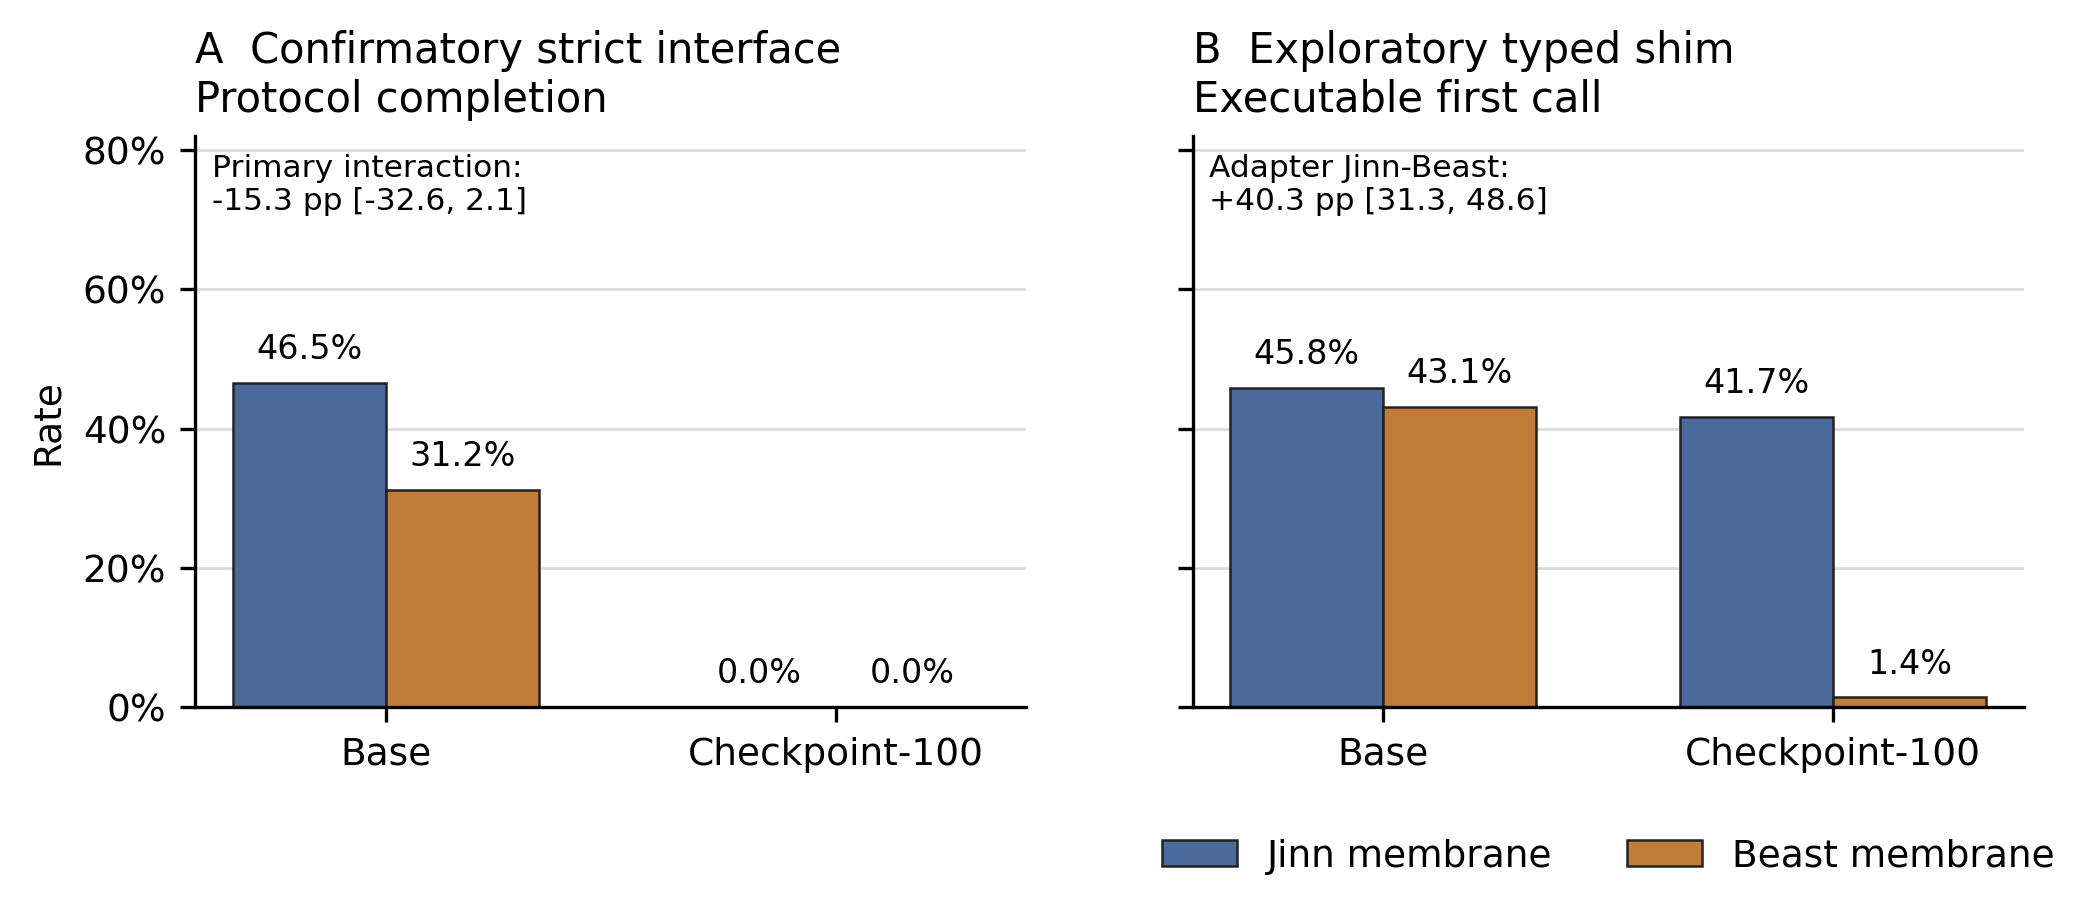
\includegraphics[keepaspectratio,alt={Confirmatory protocol completion and exploratory first-turn interface recovery}]{../experiments/jinn_persona_ambivalence_v4_expanded/control_mesh_2x2/results/control_mesh_result_figure.png}}
\caption{Confirmatory protocol completion and exploratory first-turn
interface recovery}
\end{figure}

\textbf{Figure 1.} Left: confirmatory protocol completion in the 2 × 2
factorial. Right: post-hoc first-turn recognizability and executability
under the narrow typed shim. Error bars in the underlying analysis are
family-bootstrap 95\% intervals. The exploratory interface result does
not replace the confirmatory endpoint.

\subsection{5.6 A typed shim exposed membrane-dependent recoverable
intent}\label{a-typed-shim-exposed-membrane-dependent-recoverable-intent}

Inspection of adapter outputs found a repeated serialization pattern: a
plausible JSON argument object appeared inside an opening
\texttt{\textless{}tool\_call\textgreater{}} tag, but the output omitted
the closing tag and the required
\texttt{\{"tool":\ ...,\ "arguments":\ ...\}} envelope. The strict
parser correctly rejected these calls.

We performed a post-hoc diagnostic on first turns only. The shim
accepted no prose and added no unknown values. It recognized one JSON
object only when its exact key signature uniquely identified a
registered tool, then executed the proposed call against a fresh frozen
controller.

{\def\LTcaptype{none} % do not increment counter
\begin{longtable}[]{@{}
  >{\raggedright\arraybackslash}p{(\linewidth - 6\tabcolsep) * \real{0.2000}}
  >{\raggedleft\arraybackslash}p{(\linewidth - 6\tabcolsep) * \real{0.2667}}
  >{\raggedleft\arraybackslash}p{(\linewidth - 6\tabcolsep) * \real{0.2667}}
  >{\raggedleft\arraybackslash}p{(\linewidth - 6\tabcolsep) * \real{0.2667}}@{}}
\toprule\noalign{}
\begin{minipage}[b]{\linewidth}\raggedright
Cell
\end{minipage} & \begin{minipage}[b]{\linewidth}\raggedleft
Strict first call
\end{minipage} & \begin{minipage}[b]{\linewidth}\raggedleft
Recognized after shim
\end{minipage} & \begin{minipage}[b]{\linewidth}\raggedleft
Executable after shim
\end{minipage} \\
\midrule\noalign{}
\endhead
\bottomrule\noalign{}
\endlastfoot
Base × Jinn & 0.458 & 0.458 & 0.458 \\
Base × Beast & 0.313 & 0.431 & 0.431 \\
Persona adapter × Jinn & 0.000 & 0.736 & 0.417 \\
Persona adapter × Beast & 0.000 & 0.076 & 0.014 \\
\end{longtable}
}

Within adapter weights, the Jinn-minus-Beast effect was +0.660 {[}0.556,
0.757{]} for recognizable intent and +0.403 {[}0.313, 0.486{]} for an
executable first call. The adapter × membrane interactions were +0.632
{[}0.424, 0.819{]} and +0.375 {[}0.174, 0.563{]}, respectively.

This membrane sensitivity was large despite identical adapter weights.
The Jinn prompt elicited action IDs, evidence IDs, and uniquely typed
tool arguments far more often than the Beast prompt. The result is
limited to the agent interface. Later recorded turns had been
conditioned on strict-parser rejection, so replaying them after a
repaired first call would create counterfactual trajectories and was not
done.

\section{6. Discussion}\label{discussion}

\subsection{6.1 Alignment is a composition
problem}\label{alignment-is-a-composition-problem}

The persona adapter and stateful controller were each plausible in
isolation. The adapter changed observable response form on held-out
prompts. The controller separated two decision processes under base 4B
weights. Their combination nevertheless failed completely at the strict
serialization boundary.

This result argues against treating an adapter as a drop-in ``moral
module.'' The behavior of the assembled agent depends on at least four
contracts:

\begin{enumerate}
\def\labelenumi{\arabic{enumi}.}
\tightlist
\item
  \textbf{persona contract:} what distinctions and tensions the model
  expresses;
\item
  \textbf{serialization contract:} whether the output is valid under the
  tool grammar;
\item
  \textbf{translation contract:} whether a bounded deterministic
  transducer can map the output to exactly one legal action;
\item
  \textbf{process contract:} whether accepted actions satisfy ordering,
  evidence, and commitment constraints.
\end{enumerate}

Only after these pass is it meaningful to score the final moral outcome.
A single scalar reward can hide which contract improved.

\subsection{6.2 Exogenous control was more reliable than process
self-description}\label{exogenous-control-was-more-reliable-than-process-self-description}

The v1 adapters learned a strong output contract but not the intended
frame-specific process. Version 2 achieved much larger separation with
the same 4B base weights and no additional training because process
identity was encoded in legal state transitions.

This is not an argument against RL. It is an argument for spending RL
signal on decisions the model should own. Deterministic structure should
own properties that can be specified exactly: valid tool signatures,
complete enumeration, scope, evidence-ID membership, irreversible
commitment, and critical-action caps. Model learning can then focus on
contextual judgments inside that structure.

\subsection{6.3 Dynamic and optimized membranes fail
differently}\label{dynamic-and-optimized-membranes-fail-differently}

The Jinn process created richer action interaction but more
opportunities for termination failure. At 9B, the model completed
inspection and then narrated instead of committing. In the persona
factorial, however, Jinn elicited far more recoverable action intent
than Beast.

The Beast process was shorter and generally easier to terminate, but
under the persona adapter it often collapsed into repetitive pruning
fragments without a uniquely executable call. These differences are
consistent with the operational labels: the dynamic process exposes more
decision structure, while the optimized process suppresses variation.
They should be evaluated as different control topologies, not as
symmetric system prompts.

\subsection{6.4 A safer typed-transducer
architecture}\label{a-safer-typed-transducer-architecture}

The post-hoc shim suggests a prospective architecture:

\begin{Shaded}
\begin{Highlighting}[]
\NormalTok{LLM proposes typed arguments}
\NormalTok{        ↓}
\NormalTok{deterministic transducer accepts one unique signature}
\NormalTok{        ↓}
\NormalTok{stateful controller validates IDs and transition legality}
\NormalTok{        ↓}
\NormalTok{environment executes and records the action}
\end{Highlighting}
\end{Shaded}

The transducer should be narrow. It may repair a missing wrapper only
when one exact JSON object maps to one registered tool signature. It
should reject prose, multiple objects, nested calls, extra keys, unknown
IDs, ambiguous signatures, and values not present in the current state.

This architecture does not convert the exploratory shim into
confirmatory evidence. A valid test requires fresh generation because
accepting the first call changes every later observation. The next
factorial should therefore cross strict serializer versus typed
transducer, base versus persona weights, and Jinn versus Beast membrane
on new family-disjoint tasks.

\subsection{6.5 Implications for reasoning modules and LDT
ablations}\label{implications-for-reasoning-modules-and-ldt-ablations}

Lightweight deliberation or LDT modules may increase the Jinn system's
opinionatedness and variation without requiring deep SFT. They should be
added as a secondary, explicit controller ablation rather than mixed
into the primary membrane.

A useful test would compare:

\begin{itemize}
\tightlist
\item
  Jinn adapter + plain membrane;
\item
  Jinn adapter + frozen LDT scaffold.
\end{itemize}

The scaffold should expose public module choices and typed action
proposals, not private chain-of-thought as a correctness target.
Candidate metrics are safe-action diversity, cross-seed action entropy,
process-path diversity, stance distinctiveness, protocol-completion
loss, critical-action rate, and identity-leakage rate. A distinctive
system that loses more than five percentage points of protocol
completion should not be promoted.

\subsection{6.6 What additional Prime Lab evaluation can
close}\label{what-additional-prime-lab-evaluation-can-close}

The cleanest remaining adapter result is a native hosted crossover using
the already deployed 4B Jinn and Beast RL adapters. The preregistered
closure matrix is:

{\def\LTcaptype{none} % do not increment counter
\begin{longtable}[]{@{}lll@{}}
\toprule\noalign{}
Weights & Jinn v2 membrane & Beast v2 membrane \\
\midrule\noalign{}
\endhead
\bottomrule\noalign{}
\endlastfoot
Jinn RL adapter & 96 rollouts & 96 rollouts \\
Beast RL adapter & 96 rollouts & 96 rollouts \\
\end{longtable}
}

This 384-rollout experiment would use the untouched v2 confirmatory
tasks, temperature 0, thinking disabled, 256 output tokens per turn, two
rollouts per task, and native \texttt{StatefulToolEnv} tool schemas. It
can estimate diagonal specialization, off-diagonal transfer, protocol
reliability, and the adapter × membrane interaction without the local
serializer mismatch. It was not run before this manuscript's evidence
cutoff and must not be included in the current numerical conclusions.

\section{7. Limitations}\label{limitations}

First, the frame names and source mappings are research
operationalizations whose scholar review is still pending. The paper
therefore reports system behavior under exact hash-bound treatments and
delegates broader interpretation to the repository's claim ladder.

Second, the storyworlds are authored, have three-action menus, and cover
a small number of independent families. Family-clustered intervals
prevent pseudoreplication but do not create broad external validity.

Third, the v2 development process included three prospective prompt and
schema clarifications. The confirmatory split remained untouched, but
the final result estimates performance of the clarified \texttt{0.1.15}
protocol rather than the first development draft.

Fourth, the persona primary endpoint did not pass. Checkpoint 100 was
selected by a frozen downstream rule after a positive secondary
contrast. Independent human review was absent; two learned reviewers
supplied the blinded persona scores.

Fifth, the typed-shim analysis was post hoc and first-turn only. It
diagnoses a mechanism but cannot establish complete trajectories. The
strict local serializer and Prime's native hosted tool transport are
also different interfaces, so results should not be numerically pooled
across them.

Sixth, the 9B result used the same frozen 256-token per-turn budget as
the 4B test. That is appropriate for a strict replication, but it does
not determine whether a larger budget or explicit termination affordance
would repair the 9B Jinn surface.

Finally, recovered prompt experiments lack their full raw rows and
immutable judge receipts. They are used only as motivating historical
evidence, not combined with repository-native confirmatory estimates.

\section{8. Reproducibility and evidence
map}\label{reproducibility-and-evidence-map}

The repository binds protocols, data hashes, model revisions, raw-result
hashes, analysis seeds, costs, and cleanup receipts.

{\def\LTcaptype{none} % do not increment counter
\begin{longtable}[]{@{}
  >{\raggedright\arraybackslash}p{(\linewidth - 2\tabcolsep) * \real{0.5000}}
  >{\raggedright\arraybackslash}p{(\linewidth - 2\tabcolsep) * \real{0.5000}}@{}}
\toprule\noalign{}
\begin{minipage}[b]{\linewidth}\raggedright
Evidence
\end{minipage} & \begin{minipage}[b]{\linewidth}\raggedright
Canonical artifact
\end{minipage} \\
\midrule\noalign{}
\endhead
\bottomrule\noalign{}
\endlastfoot
Persona v4 protocol &
\href{../experiments/jinn_persona_ambivalence_v4_expanded/protocol.json}{\texttt{protocol.json}} \\
Persona v4 results &
\href{../experiments/jinn_persona_ambivalence_v4_expanded/results/README.md}{\texttt{results/README.md}} \\
V2 registration &
\href{../experiments/jinn_beast_metta_rl_v1/moral_control_mesh_v2/registration.json}{\texttt{moral\_control\_mesh\_v2/registration.json}} \\
V2 deterministic signal audit &
\href{../experiments/jinn_beast_metta_rl_v1/moral_control_mesh_v2/signal_audit.json}{\texttt{signal\_audit.json}} \\
4B confirmatory receipt &
\href{../experiments/jinn_beast_metta_rl_v1/moral_control_mesh_v2/four_b_confirmatory_pass_receipt.json}{\texttt{four\_b\_confirmatory\_pass\_receipt.json}} \\
9B failure receipt &
\href{../experiments/jinn_beast_metta_rl_v1/moral_control_mesh_v2/nine_b_replication_failure_receipt.json}{\texttt{nine\_b\_replication\_failure\_receipt.json}} \\
Persona × membrane registration &
\href{../experiments/jinn_persona_ambivalence_v4_expanded/control_mesh_2x2_registration.json}{\texttt{control\_mesh\_2x2\_registration.json}} \\
Persona × membrane result receipt &
\href{../experiments/jinn_persona_ambivalence_v4_expanded/control_mesh_2x2/results/run_receipt.json}{\texttt{run\_receipt.json}} \\
Confirmatory factorial analysis &
\href{../experiments/jinn_persona_ambivalence_v4_expanded/control_mesh_2x2/results/confirmatory_analysis.json}{\texttt{confirmatory\_analysis.json}} \\
Exploratory shim analysis &
\href{../experiments/jinn_persona_ambivalence_v4_expanded/control_mesh_2x2/results/exploratory_interface_diagnostic.json}{\texttt{exploratory\_interface\_diagnostic.json}} \\
Claim scope &
\href{jinn_or_beast_claim_ladder_v1.md}{\texttt{jinn\_or\_beast\_claim\_ladder\_v1.md}} \\
\end{longtable}
}

The complete 1,152-rollout raw archive is retained at
\path{D:/Research_Engine/jinn_or_beast/jinn_persona_control_mesh_2x2};
its 100-file manifest and compressed evidence archive are hash-bound in
the result receipt. The run used one A100-SXM4-40GB pod, cost \$2.28,
and left no owned GPU process after cleanup. The persona training run
cost \$0.48 on one A6000. No local GPU was used for the reported 4B
factorial.

\section{9. Conclusion}\label{conclusion}

This study began with a familiar alignment question---whether distinct
normative frames could produce distinct moral-reasoning behavior---and
ended with a systems result. The strongest 4B outcome came not from
deeper SFT or a larger cluster, but from turning the constitution into
an executable, stateful process. Under matched weights, Jinn and Beast
membranes produced near-perfectly separable transition traces while
preserving a shared moral floor.

The result was bounded. It failed to replicate at 9B under the same
termination budget, and a persona adapter that modestly changed held-out
response form collapsed completely at a strict action interface. Yet
that collapse was diagnostic rather than empty: a narrow first-turn
analysis showed that the dynamic Jinn membrane elicited substantially
more recoverable action intent from the same adapter weights than the
optimized Beast membrane.

The practical lesson is to design moral agents as layered systems. Let
model weights supply contextual judgment and voice. Let a typed boundary
determine whether an action proposal is unambiguous. Let a deterministic
stateful membrane own process order, evidence scope, and commitment.
Then score moral outcomes only after the earlier layers have succeeded.
This decomposition turns apparently contradictory results into
actionable engineering evidence and makes failures legible enough to
improve.

\section{References}\label{references}

\begin{enumerate}
\def\labelenumi{\arabic{enumi}.}
\tightlist
\item
  Bai, Y., et al.~(2022). ``Constitutional AI: Harmlessness from AI
  Feedback.'' \href{https://arxiv.org/abs/2212.08073}{arXiv:2212.08073}.
\item
  Ouyang, L., et al.~(2022). ``Training Language Models to Follow
  Instructions with Human Feedback.''
  \href{https://arxiv.org/abs/2203.02155}{arXiv:2203.02155}.
\item
  Yao, S., et al.~(2023). ``ReAct: Synergizing Reasoning and Acting in
  Language Models.''
  \href{https://arxiv.org/abs/2210.03629}{arXiv:2210.03629}.
\item
  Schick, T., et al.~(2023). ``Toolformer: Language Models Can Teach
  Themselves to Use Tools.''
  \href{https://arxiv.org/abs/2302.04761}{arXiv:2302.04761}.
\item
  Soni, H. (2026). ``ToolFailBench: Diagnosing Tool-Use Failures in LLM
  Agents.'' \href{https://arxiv.org/abs/2607.04686}{arXiv:2607.04686}.
\item
  OpenCog Hyperon. ``The MeTTa Programming Language.''
  \href{https://hyperon.opencog.org/}{Project documentation}.
\item
  Yang, A., et al.~(2025). ``Qwen3 Technical Report.''
  \href{https://arxiv.org/abs/2505.09388}{arXiv:2505.09388}.
\end{enumerate}

\section{Appendix A. Frozen gate
definitions}\label{appendix-a.-frozen-gate-definitions}

The 4B v2 confirmatory gate required all of:

\begin{itemize}
\tightlist
\item
  protocol completion ≥ 0.90;
\item
  executed-process margin ≥ 0.80;
\item
  safe-tie paired target rate ≥ 0.70;
\item
  decisive convergence ≥ 0.85;
\item
  shared moral quality ≥ 0.82;
\item
  grounded commit rate ≥ 0.80;
\item
  efficient trace rate ≥ 0.75;
\item
  rejected tool-event fraction ≤ 0.10;
\item
  critical final action rate = 0;
\item
  truncation rate ≤ 0.05.
\end{itemize}

The persona × membrane adapter non-inferiority gate required the lower
family-bootstrap bound to remain above −0.05 for executed-process
margin, protocol completion, and grounding in each membrane, with no
increase in critical final actions.

\section{Appendix B. Evidence-status
language}\label{appendix-b.-evidence-status-language}

To preserve the prospective record, the manuscript uses:

\begin{itemize}
\tightlist
\item
  \textbf{confirmatory} only for frozen endpoints on untouched
  evaluation families;
\item
  \textbf{development-only} for online learning curves and held-out sets
  used for promotion decisions;
\item
  \textbf{recovered} for session-extracted summaries lacking complete
  canonical row bundles;
\item
  \textbf{exploratory} for analyses defined after outcome inspection;
\item
  \textbf{planned} for registered experiments with no outputs at the
  evidence cutoff.
\end{itemize}

The native Prime adapter crossover and LDT scaffold ablation remain
planned. No result from either is represented in this draft.

\end{document}
